{\setbeamercolor{palette primary}{bg=ExColor}
	\begin{frame}[fragile]{Aufgabe}
		\metroset{block=fill}
		\begin{alertblock}{Die folgende Induktion zeigt eine seltsame Aussage.}
			Ist der Beweis korrekt geführt? Was ist passiert?
		\end{alertblock}
		\metroset{block=transparent}
		Sei $A(n)\defeq$ In einer Herde aus $n$ Telefonen haben alle die selbe Farbe.
		Zu zeigen: $A(n)$ gilt für alle $n \in \mathbb{N}^+$.
		\begin{alertblock}{Induktionsanfang IA}
			$A(1)$: Aussage gilt für $n\defeq 1$, da ein Telefon nur eine Farbe haben kann.
		\end{alertblock}
		\begin{alertblock}{Induktionsvorraussetzung IV}
			Ang. $A(n)$ gilt für $n\geq1$.
		\end{alertblock}
		\begin{alertblock}{Induktionsschritt IS}
			Zeige Aussage gilt für alle $n+1$ unter Nutzung der I.V.\\
			d.h. wir zeigen $A(n+1)=$ In einer Herde aus $n+1$ Telefonen haben alle die selbe Farbe.
		\end{alertblock}
	\end{frame}
	\begin{frame}[fragile]{Aufgabe}
		\footnotesize{
			\begin{alertblock}{Induktionsschritt IS}
				Wir betrachten eine Herde aus $n+1$ Telefonen:
				\[\underbrace{\text{\Telefon}\text{\Telefon}\text{\Telefon}\text{\Telefon}\text{\Telefon}\dots\text{\Telefon}\text{\Telefon}}_{n+1}\]
				Wir sondern ein Telefon aus und betrachten den Rest. Nach I.V. haben diese alle die selbe Farbe.
				\[\underbrace{\alert{\text{\Telefon}\text{\Telefon}\text{\Telefon}\text{\Telefon}\text{\Telefon}\dots\text{\Telefon}}}_{n}\text{\Telefon}\]
				Jetzt sondern wir ein anderes Telefon aus.
				\[\alert{\text{\Telefon}}\underbrace{\alert{\text{\Telefon}\text{\Telefon}\text{\Telefon}\text{\Telefon}\dots\text{\Telefon}}\text{\Telefon}}_{n}\]
				Die übrigen $n$ Telefone haben nach I.V. wieder die selbe Farbe.
				\[\underbrace{\alert{\text{\Telefon}\text{\Telefon}\text{\Telefon}\text{\Telefon}\text{\Telefon}\dots\text{\Telefon}\text{\Telefon}}}_{n+1}\]
				Also haben alle $n+1$ Telefone die selbe Farbe.
				$\leadsto$ $A(n)$ gilt für alle $n$.
			\end{alertblock}
		}
	\end{frame}
}

{\setbeamercolor{palette primary}{bg=ExColor}
	\begin{frame}[fragile]{Lösungen}
		\small{
			\metroset{block=fill}
			\begin{block}{Das Problem}
				Die Vorangehensweise erfordert, dass die betrachteten Mengen an $n$ Telefonen mindestens ein gemeinsames Element haben. Sie teilen dann die Farbe dieses Elements. Allerdings gibt es ein überlappendes Element erst ab $3$ Telefonen.
				\[
					\color{mLightGreen}A(1) \overset{\text{I.V.}}{\implies}
					\alert{A(2):\overbrace{\text{\Telefon}}\underbrace{\text{\Telefon}}} \color{black} \overset{\alert{\text{I.V.}}}{\nimplies}
					A(3):\rlap{$\overbrace{\phantom{\text{\Telefon\Telefon}}}$}\text{\Telefon}\underbrace{\text{\Telefon\Telefon}} 
					\overset{\alert{\text{I.V.}}}{\nimplies} \dots \overset{\alert{\text{I.V.}}}{\nimplies} A(n)
				\]
				Die Kette an verifiziert wahren Aussagen ist also unterbrochen, da es keine gültige Vorraussetzung gibt um $A(2+1)$ zu zeigen.
			\end{block}
		}
	
		\begin{figure}
		\resizebox{.6\textwidth}{!}{
			\centering%
			\begin{subfigure}{0.3\textwidth}
				\centering%
				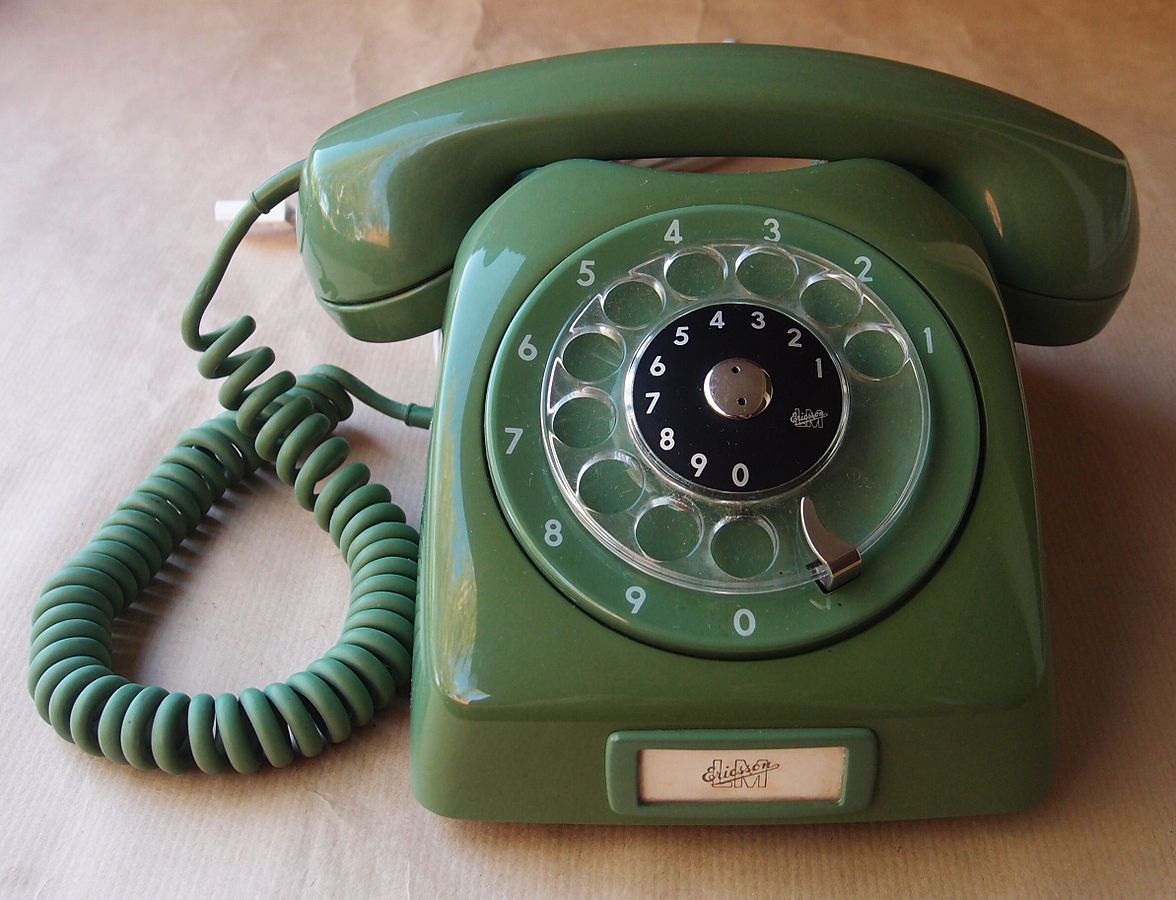
\includegraphics[height=0.5in]{../figures/green.jpg}
				\caption{grünes Telefon}
			\end{subfigure}
			$\qquad$
			\begin{subfigure}{0.3\textwidth}
				\centering%
				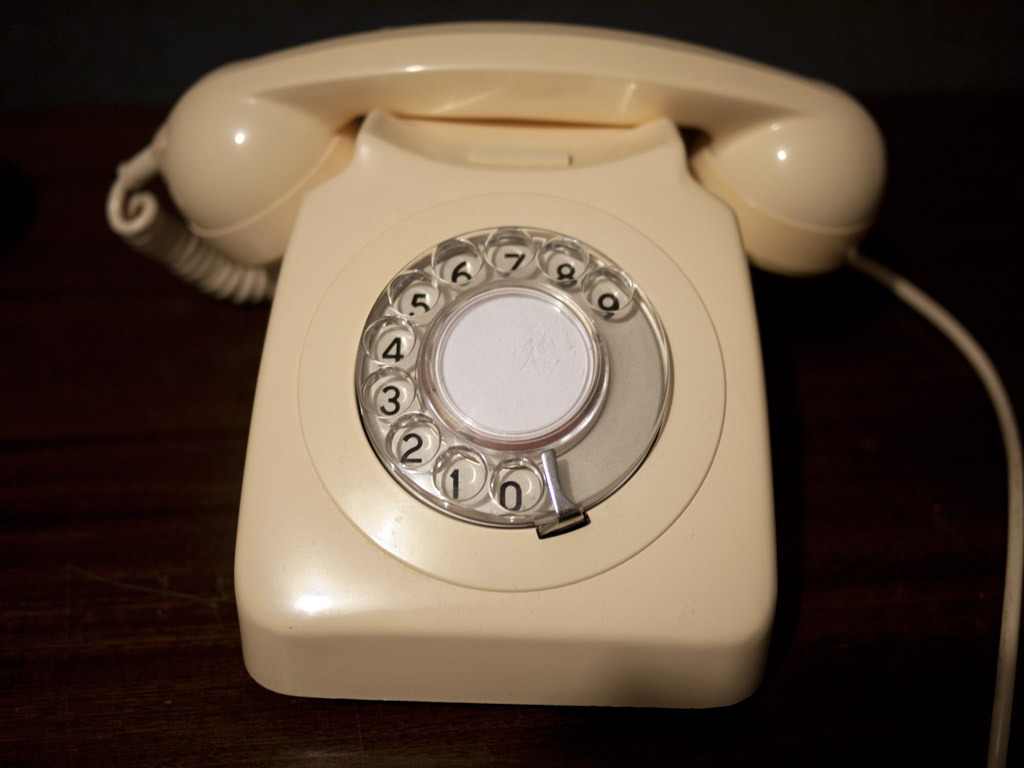
\includegraphics[height=0.5in]{../figures/white.jpg}
				\caption{weißes Telefon}
			\end{subfigure}
		}
			\caption{Telefone mit unterschiedlicher Farbe\footnote{\tiny{Quelle: https://commons.wikimedia.org/}}}
		\end{figure}
	\end{frame}
}